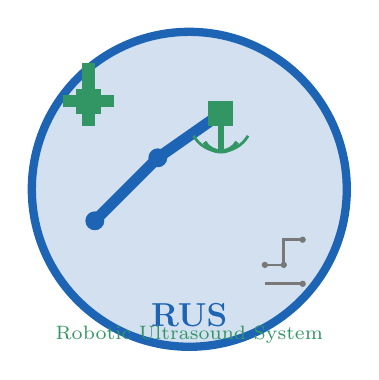
\begin{tikzpicture}[scale=0.8]
    % Define colors
    \definecolor{robotblue}{RGB}{30,100,180}
    \definecolor{medicalgreen}{RGB}{50,150,100}
    \definecolor{techgray}{RGB}{120,120,120}
    
    % Main circle background
    \fill[robotblue!20] (0,0) circle (2.5);
    \draw[robotblue, line width=3pt] (0,0) circle (2.5);
    
    % Robotic arm representation
    \draw[robotblue, line width=4pt] (-1.5,-0.5) -- (-0.5,0.5) -- (0.5,1.2);
    \fill[robotblue] (-1.5,-0.5) circle (0.15);
    \fill[robotblue] (-0.5,0.5) circle (0.15);
    \fill[robotblue] (0.5,1.2) circle (0.15);
    
    % Ultrasound probe
    \fill[medicalgreen] (0.3,1.0) rectangle (0.7,1.4);
    \draw[medicalgreen, line width=2pt] (0.5,1.0) -- (0.5,0.6);
    
    % Ultrasound waves
    \draw[medicalgreen, line width=1.5pt] (0.5,0.6) arc[start angle=270, end angle=210, radius=0.3];
    \draw[medicalgreen, line width=1.5pt] (0.5,0.6) arc[start angle=270, end angle=330, radius=0.3];
    \draw[medicalgreen, line width=1pt] (0.5,0.6) arc[start angle=270, end angle=210, radius=0.5];
    \draw[medicalgreen, line width=1pt] (0.5,0.6) arc[start angle=270, end angle=330, radius=0.5];
    
    % Medical cross
    \fill[medicalgreen] (-1.8,1.2) rectangle (-1.4,1.6);
    \fill[medicalgreen] (-1.8,1.2) rectangle (-1.4,1.6);
    \fill[medicalgreen] (-1.7,1.0) rectangle (-1.5,2.0);
    \fill[medicalgreen] (-2.0,1.3) rectangle (-1.2,1.5);
    
    % Technology elements (circuit pattern)
    \draw[techgray, line width=1pt] (1.2,-1.2) -- (1.5,-1.2) -- (1.5,-0.8) -- (1.8,-0.8);
    \draw[techgray, line width=1pt] (1.2,-1.5) -- (1.8,-1.5);
    \fill[techgray] (1.2,-1.2) circle (0.05);
    \fill[techgray] (1.5,-1.2) circle (0.05);
    \fill[techgray] (1.8,-0.8) circle (0.05);
    \fill[techgray] (1.8,-1.5) circle (0.05);
    
    % Text elements
    \node[robotblue, font=\bfseries\large] at (0,-2.0) {RUS};
    \node[medicalgreen, font=\scriptsize] at (0,-2.3) {Robotic Ultrasound System};
\end{tikzpicture}
